\section{Лекция 6. Полиэдральный конус }
\subsection{Полиэдральный конус}

\noindent\textbf{Определение 2.40}\\
Полиэдральный конус - это конус, который является полиэдром.\\

\subsection{Свойства полиэдрального конуса}

\noindent\textbf{Замечание 2.41}\\
Множество  $K\subseteq \mathbb{R}^{m\times n}$ ~--- полиэдральный конус тогда и только тогда, когда $\exists A\in\mathbb{R}^{m\times n}$, удовлетворяющее условию
\begin{equation*}
K=P^{\leq}\left(A,\mathbb{O}_{n}\right)=\{x|Ax\leq\mathbb{O}_{n}\}
\end{equation*}

\noindent\textbf{Замечание 2.42}\\
Полиэдральный конус выпуклый и замкнутый. \\

\noindent\textbf{Замечание 2.43}\\
Поляры конечно порожденных конусов являются полиэдральными конусами. \\

\subsection{Теоремы и леммы про полиэдральные конусы}

\noindent\textbf{Лемма 2.44}\\
Каждый полиэдральный конус является конечно порожденным.\\
(Смотри картинку ниже, черные линии - вектора для выпуклой конической оболочки)
\begin{center}
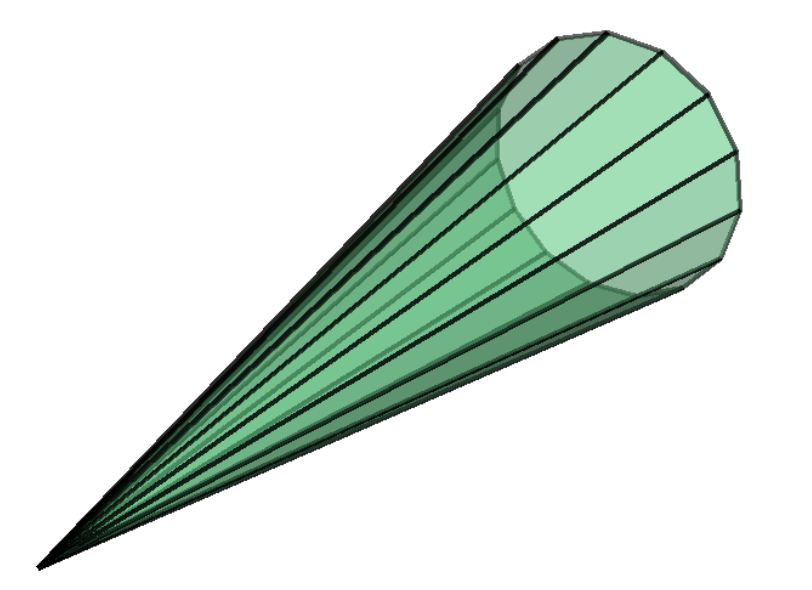
\includegraphics[scale=0.3]{polyed.png}
\end{center}
\noindent\textbf{Теорема 2.45}\\
Конус полиэдральный тогда и только тогда, когда он конечно порожденный.\\
$\blacktriangleleft$
\begin{itemize}
\item  Покажем, что каждый конечно порожденный конус $K$ является полиэдральным.
\item Пусть $K$ конечно порожденный конус
\begin{itemize}
\item $\Longrightarrow K^{\circ}$ полиэдральный (следует из замечания 2.43).
\item $\Longrightarrow K^{\circ}$ конечно порожденный (следует из леммы 2.44).
\item $\Longrightarrow K^{\circ\circ}$ полиэральный конус (следует из замечания 2.43).
\end{itemize}
\item Покажем, что $K=K^{\circ\circ}$.
\item $K$ выпуклый, замкнутый $\Longrightarrow K=K^{\circ\circ}$(следует из теоремы 2.32, 2.38).
\end{itemize}
$\blacktriangleright$

\subsection{Усиление Леммы 2.44}
\noindent\textbf{Определение}\\
$\forall M \in \mathbb{R}^{m\times n}$ слудующие множества:
\begin{itemize}
\item $\vartriangleright \delta(M)=\{det M_{I\times J}| I\subseteq[m], J\subseteq[n],|I|=|J|\}$. Судя по описанию, это -- множество миноров в матрице $M$.
\item $\vartriangleright \Delta(M)=\{\frac{p}{q}| p,q \in\delta(M)\cup(-\delta(M)), q\neq0\}$ -- множество дробей, что числитель и знаменатель лежат в указанных множествах миноров, причем $q\neq 0$.
\end{itemize}
\noindent\textbf{Лемма $2.44^{\ast}$}\\
$\forall A\in\mathbb{R}^{m\times n},\exists X \subseteq\Delta(A)^{n}, |X|<\infty$ такое, что $\{x|Ax<0\}=ccone(X)$.\\
($\Delta(A)^{n}$ по логике означает n-кратное декартово произведение множества $\Delta(A)$).\\

\noindent\textbf{Замечания к $\Delta(M)$}
\begin{itemize}
\item $M\in \mathbb{Q}^{m\times n} \Longrightarrow \Delta(M)\subseteq \mathbb{Q}.$
\item Определим понятие \textbf{Длины кода}:
\begin{itemize}
\item $a\in \mathbb{Q}, a=\frac{p}{q}, p \in \mathbb{Z},q \in \mathbb{N}/\{0\}, p, q$ взаимно простые:$ <a>:=1+[\log_{2}(|p|+1)]+[\log_{2}(q+1)]. \text{ } \left\langle\right\rangle$--длинна кода.
\end{itemize}
\begin{itemize}
\item Количество бит для хранения вектора $v\in \mathbb{Q}^{n}: <v>:=n+\sum\limits_{i=1}^n<v_{i}>.$
\end{itemize}
\begin{itemize}
\item Количество бит для хранения матрицы $M \in \mathbb{Q}^{m\times m}: <M>:=mn+\sum\limits_{i=1}^n \sum\limits_{j=1}^m<M_{ij}>$
\end{itemize}
\end{itemize}
\begin{itemize}
\item Максимальная длинна кода в матрице $max\{<z>: z\in \Delta(M)\}$ ограничена полиномом от длины кода матрицы $M \;  \forall M \; \in \mathbb{Q}^{m\times n}$
\end{itemize}

\noindent\textbf{Для доказательства Леммы $2.44^{\ast}$:}\\
В лемме $2.44^{\ast}$ важно показать, что $X\subseteq \Delta(A)^{n}$.\\
Индукция по $p=0, 1, ...$:\\
Для всех $B\in \mathbb{R}^{p\times n}, C \in \mathbb{R}^{q\times n} (p+q\geq1, n\geq1), A =\begin{pmatrix} B\\C \end{pmatrix}\in \mathbb{R}^{(p+q)\times n}, \exists X \subseteq \Delta(A)^{n}, |X|<\infty$, такое что $K:=\{ x\in \mathbb{R}^{n}| Bx\leq0, Cx=0\}=ccone X$.\\

\noindent\textbf{Лемма 2.44а}\\
Пусть $B\in \mathbb{R}^{p\times n}, C \in \mathbb{R}^{q\times n} (p+q\geq1, n\geq1), A =\begin{pmatrix} B\\C \end{pmatrix}\in \mathbb{R}^{(p+q)\times n},\\ K:=\{x\in \mathbb{R}^{n}|Bx<=0,Cx=0\}.$
\begin{itemize}
\item В случае, если $dim(Ker(A))\geq dim(Ker(C))-1: \exists X\subseteq \Delta(A)^{n}, |X|<\infty$, такое что $K=ccone X$.
\end{itemize}
\begin{itemize}
\item  В противном случае $\exists z\in Ker(C)$, такое что $z\notin K, -z\notin K$.
\end{itemize}
\begin{center}
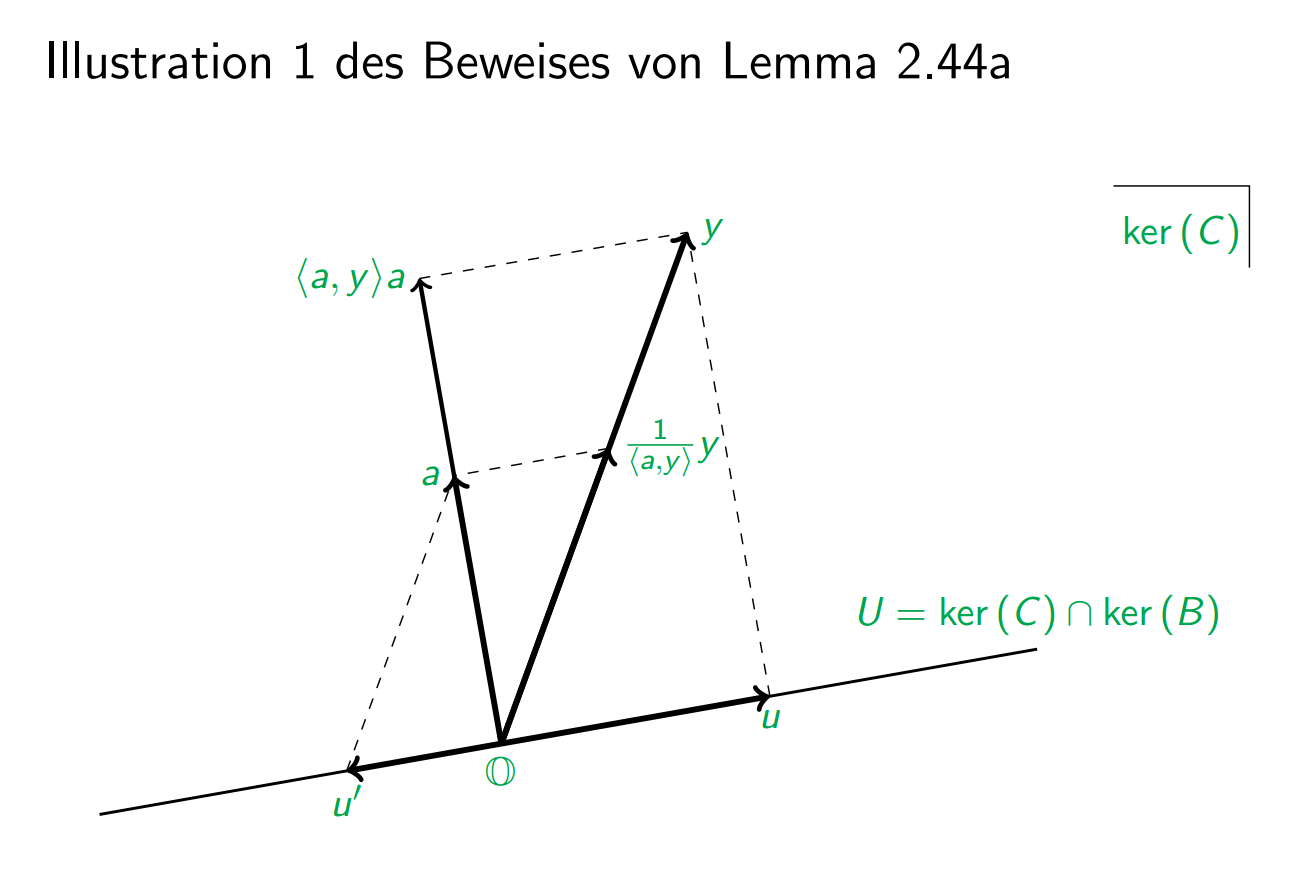
\includegraphics[scale=0.4]{lm244a.png}
\end{center}
\begin{center}
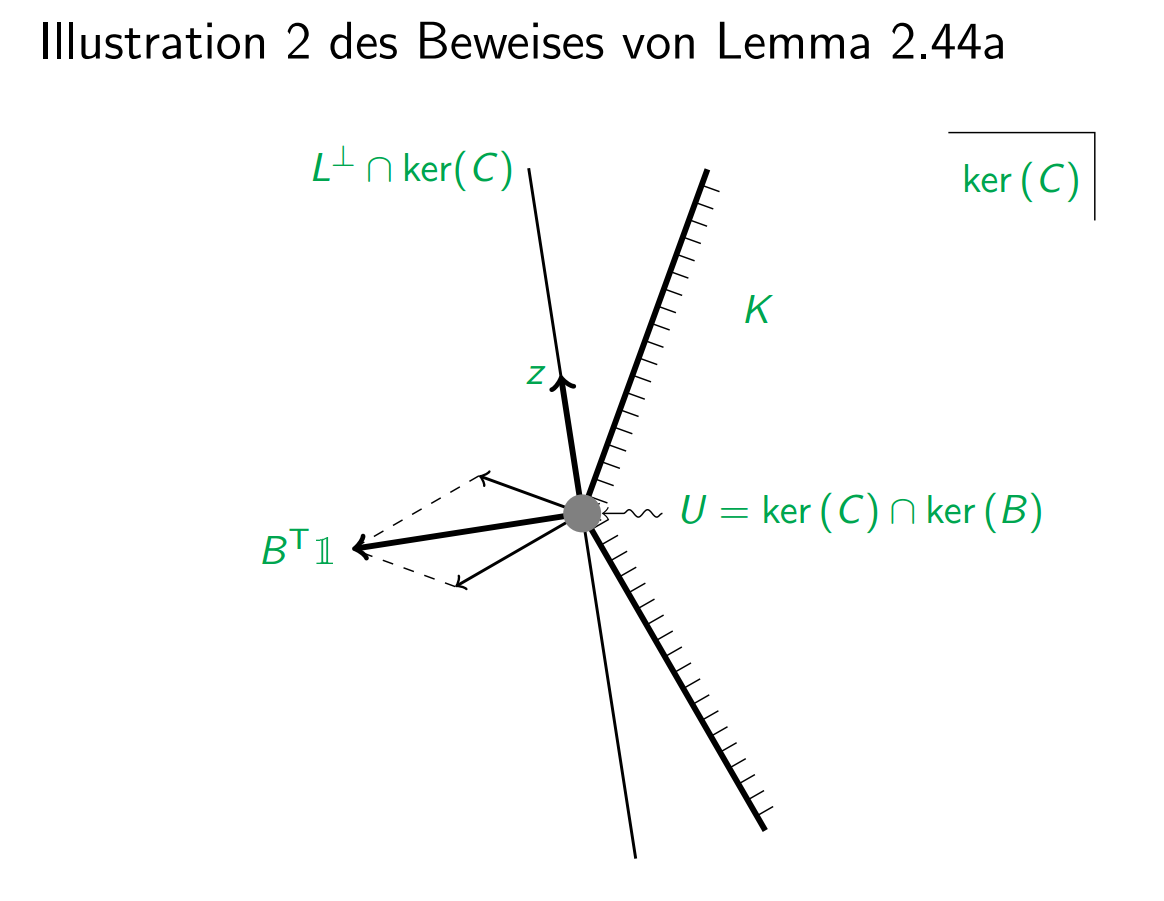
\includegraphics[scale=0.4]{lm244a2.png}
\end{center}
\newpage
\noindent\textbf{Докажем лемму $2.44^{\ast}$ по индукции}\\
\begin{itemize}
\item $p=0$: Доказательство вытекает из Леммы 2.44а
\end{itemize}
\begin{itemize}
\item $p\geq1$: из Леммы 2.44а следует, что можно принять $z\in Ker(C)$, такое что $z,-z\notin K$.
\begin{itemize}
\item Для всеx $i\in [p]: B^{(i)} \in \mathbb{R}^{(p-1)\times n}, K_{i}:=\{x\in\ \mathbb{R}^{n}:B^{(i)}x\leq0, \\<B_{i,\ast},x>=0,Cx=0\}$.
\end{itemize}
\begin{itemize}
\item По индукционному предположению $\exists X_{i}\subseteq \Delta(A)^{n},|X_{i}|<\infty$, такое что $K_{i}=ccone X_{i}$.\\
Достаточно показать, что $K\subseteq cconeX, X:=\cup_{i=1}^p X_{i}$("$\supseteq$" очевидно).
\end{itemize}
\begin{itemize}
\item Пусть $x\in K$.
\end{itemize}
\begin{itemize}
\item $I:=\{i\in[p]: <B_{i,\ast},z> >0\}\neq0$ (т.к. $Bz\leq0, Cz=0, z\notin K$)
\end{itemize}
\begin{itemize}
\item $\forall i\in I: \lambda_{i}:=max\{\lambda\geq0: <B_{i,\ast},x+\lambda z>\leq0\}\geq0 (Bx\leq0$, т.к. $x\in K$).
\end{itemize}
\begin{itemize}
\item Выберем $i^{\ast}\in I, \lambda^{\ast}:=\lambda_{i^{\ast}}=min\{\lambda_{i},i\in I\}\geq0$.\\
Тогда $B(x+\lambda^{\ast}z)\leq0$ (т.к. $Bx\leq0$), $<B_{i^{\ast},\ast},x+\lambda^{\ast}z>=0, C(x+\lambda^{\ast}z)=0\;(Cx=0,Cz=0)$.
\end{itemize}
\begin{itemize}
\item $\Longrightarrow x+\lambda^{\ast}z \in K_{i^{\ast}}=ccone X_{i^{\ast}}\subseteq ccone X, \lambda^{\ast}\geq0$
\end{itemize}
\begin{itemize}
\item Аналогично: для $-z \in Ker C\backslash K, \mu^{\ast}\geq0$ можно построить $x+\mu^{\ast}(-z) \in ccone X$\\
$\Longrightarrow x-\mu^{\ast}z \in ccone X, \mu^{\ast}\geq0$
\end{itemize}
\begin{itemize}
\item Т.к. $ccone X$ выпуклый, то \\
$x=\frac{\mu^{\ast}}{\lambda^{\ast} + \mu^{\ast}}(x+\lambda^{\ast}z)+\frac{\lambda^{\ast}}{\lambda^{\ast}+\mu^{\ast}}(x-\mu^{\ast}z) \in ccone X$, т.к. является выпуклой комбинацией двух точек, ему принадлежащих.
\end{itemize}
\end{itemize}
\begin{center}
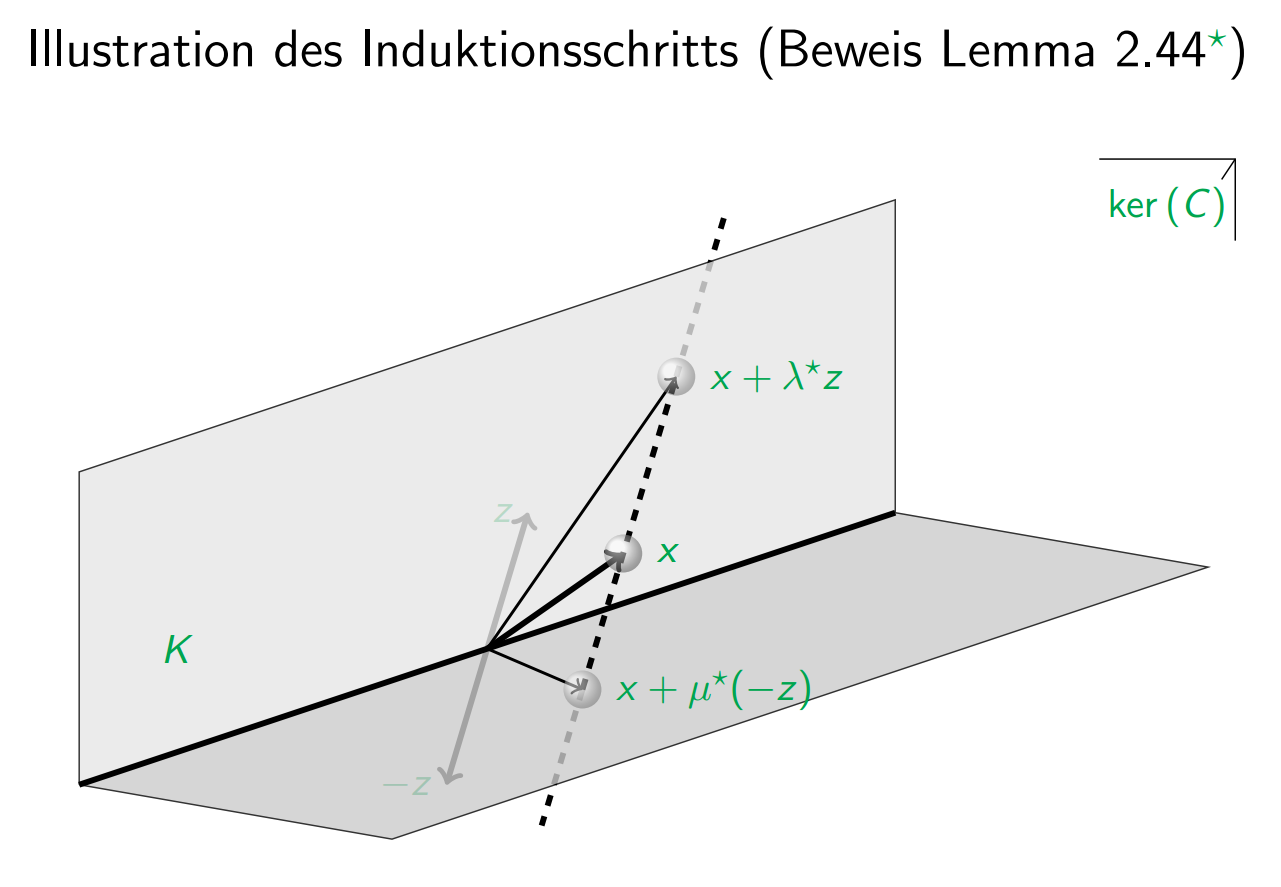
\includegraphics[scale=0.4]{lm244ast.png}
\end{center}
